%% ============================================================
%% Breaking the Bubble? — MERGED & SHORTENED DRAFT (August 2026)
%%
%% This file merges NEWAIBubble.tex (framing and wording: general
%% relevance, disasters as an extreme case, four key messages) with
%% DisasterAIFilter_main.tex (NHB structure, updated results from
%% workflow run 32040117179, cognitive-gap sweep run 32113082707,
%% Methods), shortened to Nature Human Behaviour article length
%% (~4,000 words main text; 6 figures + 1 table in the main text).
%% The full-length merged version is in git history (commit 44db40b).
%%
%% Four gaps in the Introduction map one-to-one onto four findings.
%%
%% MOVED TO SUPPLEMENTARY (beyond the full-length draft's moves):
%%   paired per-seed delta table  -> Supplementary Table S11
%%   alpha_star_sensitivity.png   -> Supplementary Fig. S6
%%   aeci_evolution.png           -> Supplementary Fig. S7
%%   promises/perils table        -> Supplementary Table S10
%%
%% CITATIONS: no new references; all keys verified against
%% References.bib (audit 2026-08-18).
%% ============================================================

\documentclass[pdflatex,sn-nature]{sn-jnl}

\usepackage{graphicx}
\graphicspath{{Figures/}{./}}
\usepackage{multirow}
\usepackage{amsmath,amssymb,amsfonts}
\usepackage{amsthm}
\usepackage{booktabs}
\usepackage{tikz}
\usetikzlibrary{arrows.meta,positioning,calc}

\begin{document}

\title[Breaking the Bubble?]{Breaking the Bubble? How Belief-Aligned AI Reshapes Collective Opinions and Decisions in Urgent Situations}

\author*[1,2]{\fnm{Tina} \sur{Comes}}\email{t.comes@tudelft.nl}

\affil*[1]{\orgdiv{Faculty of Technology, Policy \& Management}, \orgname{TU Delft}, \orgaddress{\city{Delft}, \country{The Netherlands}}}
\affil[2]{\orgdiv{Institute for the Protection of Terrestrial Infrastructures}, \orgname{DLR}, \orgaddress{\city{Sankt Augustin}, \country{Germany}}}

\abstract{In an increasingly fragmented world, AI promises to break echo chambers by giving everyone access to information. Yet information that contradicts beliefs risks rejection, and AI trained on human feedback drifts towards sycophancy: confirming what its users already believe. Evidence on belief-aligned AI comes from individuals interacting with a single AI, yet echo chambers form in networks. Here we couple an agent-based model of disaster response -- an extreme case in which urgent decisions leave little room for verification -- to an AI whose reports vary, through an alignment parameter $\alpha$, from ground truth to full confirmation. Interaction structure decides the influence of AI: a confirming AI deepens social echo chambers only where information access follows social ties. A fully truthful AI creates echo chambers of its own, converging the beliefs of its most reliant users. An interior alignment optimum therefore exists only under network-bounded access ($\alpha^{*} \approx 0.3$--$0.5$ once decision quality is accounted for), with existence and location set by the population's cognitive profile. Rising alignment concentrates harm on those remote from the events, who withdraw from the response; central network positions offer no protection. Alignment and sycophancy are thus properties of the sociotechnical system, not of the model alone.}

\keywords{Sycophancy, AI Alignment, Echo Chamber, Filter Bubble, Opinion Dynamics, Human--AI Interaction, Agent-Based Modelling, Disaster Response}

\maketitle

\section{Introduction}\label{sec:intro}

Societies are fragmenting into segregated information spaces. Online and offline, echo chambers form: information environments in which pre-existing beliefs are reinforced while exposure to diverse or contradictory perspectives is limited \citep{mahmoudi2024echo}, with polarisation and the erosion of shared factual ground as consequences \citep{jeon2024hearhere,cinelli2021echo,bail2018exposure,baumann2020modeling}. Into this landscape, artificial intelligence (AI) arrives. As we humans increasingly delegate the collection, analysis and interpretation of information to AI systems \citep{klingbeil2024trust}, the promise is that these systems give everyone access to accurate and tailored information beyond their own circles, correcting the biases and bridging the divides that human information sharing produces \citep{jeon2024hearhere}.

This promise collides with how such systems are built. Information that contradicts prior beliefs risks being rejected, and rejection erodes trust in the source \citep{glikson2020human}. AI systems are therefore optimised on human approval: preference-based training, most prominently reinforcement learning from human feedback, tunes outputs towards responses that raters reward \citep{christiano2017deep,ouyang2022training}. Because raters prefer responses that match their own views, this produces sycophancy -- a drift towards confirming the user's beliefs, documented across AI assistants \citep{sharma2023sycophancy,sharma2024generative} and shown to decrease pro-social behaviour \citep{cheng2026sycophantic}. An AI that overly tunes into existing beliefs risks amplifying the very echo chambers it promises to break \citep{ekstrom2022self} -- the alignment paradox \citep{west2025alignment}. The question thus becomes: how far should AI align with human beliefs in order to be accepted and used, without forfeiting the correction it promises?

This dilemma is most acute in urgent decision situations, where high-stakes decisions must be taken under time pressure and uncertainty, leaving little room for reflection, deliberation and verification \citep{svenson1993time,mendonca2001decision,comes2020coordination}. Crises and disasters concentrate these features like no other setting: fuelled by climate change, inequalities and conflict, polycrises erode progress towards sustainability \citep{sogaard2024evolution}, and digital tools -- from remote sensing to anticipatory action and agentic decision support -- are promoted precisely as the way to collect, analyse and act on crisis information at a speed and scale humans cannot match \citep{qadir2016crisis,voigt2007satellite,reichstein2025early,acharya2025agentic} (an overview of promises and perils is given in Supplementary Table~S10). We therefore study disasters as an extreme case: the setting in which the mechanisms coupling AI alignment to collective beliefs and decisions appear in their sharpest form, in which misallocated attention translates directly into unmet needs, and from which lessons can be drawn for the many milder settings that share its ingredients.

Whether alignment amplifies or corrects, however, is not decided between one user and one AI, because beliefs form in networks. Individuals interact preferentially with others whose opinions lie within a bounded range of their own \citep{hegselmann2002opinion}, align their opinions with their peers \citep{friedkin1999social}, and associate homophilously with those who share their beliefs \citep{mcpherson2001birds}; weak ties that bridge otherwise separate groups are the principal channel through which novel information enters \citep{granovetter1973strength,Gillani2018}. Crises tighten every one of these mechanisms: sensemaking under uncertainty is a social process \citep{weick2005organizing,klein2010rapid}, people fall back on their immediate vicinity and close groups and display selective exposure and confirmation bias \citep{comes2020coordination,barbera2015tweeting,paulus2024interplay}, disasters disrupt the infrastructures that carry information \citep{holguin2012unique}, and the resulting silos are amplified by a focus on nearby suffering at the expense of cascading effects further away \citep{pan2012crisis,wolbers2018introducing}. Yet the evidence on belief-aligned AI does not reach this collective level: sycophancy has been characterised for individual model responses and in repeated interaction between one human and one AI \citep{sharma2024generative,zhang2024see,glickman2024human}, while social influence in networks is known to reshape collective accuracy in ways that individual-level analysis cannot reveal \citep{lorenz2011social,becker2017network}. This paper therefore asks: \emph{Does AI act as a bridge that breaks echo chambers by providing broader perspectives, or does it instead reinforce existing filter bubbles through its alignment mechanisms -- and under which structural conditions does either occur?}

To answer it, we use an agent-based model of decentralised disaster relief in which heterogeneous human agents form beliefs about an evolving disaster by combining local observation with queries to peers or to an AI whose reports vary, through an alignment parameter $\alpha$, between ground truth and full confirmation. Agents accept or reject information, update their beliefs, act on them by sending relief, and learn from the delayed outcomes which sources to consult next. The model builds on established opinion-dynamics frameworks \citep{deffuant2000mixing,hegselmann2002opinion} and captures prototypical decision-making under uncertainty through confirmation-seeking \emph{exploitative} and accuracy-seeking \emph{exploratory} agents \citep{march1991exploration,comes2020coordination}. Four research gaps structure the study. First, empirical accounts of crisis communication describe information access bounded by network ties and location \citep{pan2012crisis,holguin2012unique,granovetter1973strength}, yet models of algorithmic influence on opinion dynamics grant agents unrestricted access and treat the structure as fixed; the structural conditions under which a belief-aligned AI amplifies or breaks echo chambers have not been isolated (Gap~1). Second, because trust in crises is swift, built on roles and expectations rather than experience \citep{tatham2010application,kaplan2023trust,manzini2024should}, alignment becomes the operative route to adoption \citep{glikson2020human,lee2004trust} -- but a fully truthful AI is not automatically the remedy: when many users consult a shared source, its heaviest users may converge on its estimates, including its errors, regardless of their social ties, so whether collective harm is monotonic in alignment or interior alignment levels balance adoption against distortion is open (Gap~2). Third, in urgent situations beliefs translate immediately into actions whose outcomes feed back into information collection \citep{gralla2016problem,march1991exploration}; how echo chambers and collective decision performance co-evolve through this loop cannot be extrapolated from dyadic findings (Gap~3). Fourth, actors remote from the events depend entirely on mediated information \citep{holguin2012unique,comes2020coordination}, yet the equity debate in humanitarian AI centres on data and algorithmic bias rather than on networks \citep{coleman2024weaving,beduschi2022harnessing}; how the harms of belief-alignment are distributed across space and the network has not been studied (Gap~4).

The model operationalises these gaps as follows (Fig.~\ref{fig:concept}; full specification in the Methods). A population of human agents, organised in homophilous communities \citep{mcpherson2001birds}, forms beliefs about an evolving disaster; AI agents answer queries with reports that a single parameter $\alpha \in [0,1]$ interpolates between ground truth ($\alpha = 0$) and confirmation of the querier's community beliefs ($\alpha = 1$), tracing the dose--response relationship of Gap~2. Every sweep is run under two configurations that differ only in whether access is structurally bounded -- a \emph{main model}, in which agents move through the disaster space and queries follow the ties of a spatially embedded social network, and a \emph{control}, in which agents are immobile and anyone can consult any other -- contrasted on identical random seeds to isolate the structural conditions of Gap~1. Beliefs drive relief decisions whose delayed rewards shape future source selection, and all outcomes are measured at the level of communities and the population (Gap~3) and decomposed by position in space and network (Gap~4). The Results present one finding per gap.

\begin{figure}[h]
\centering
\resizebox{\textwidth}{!}{%
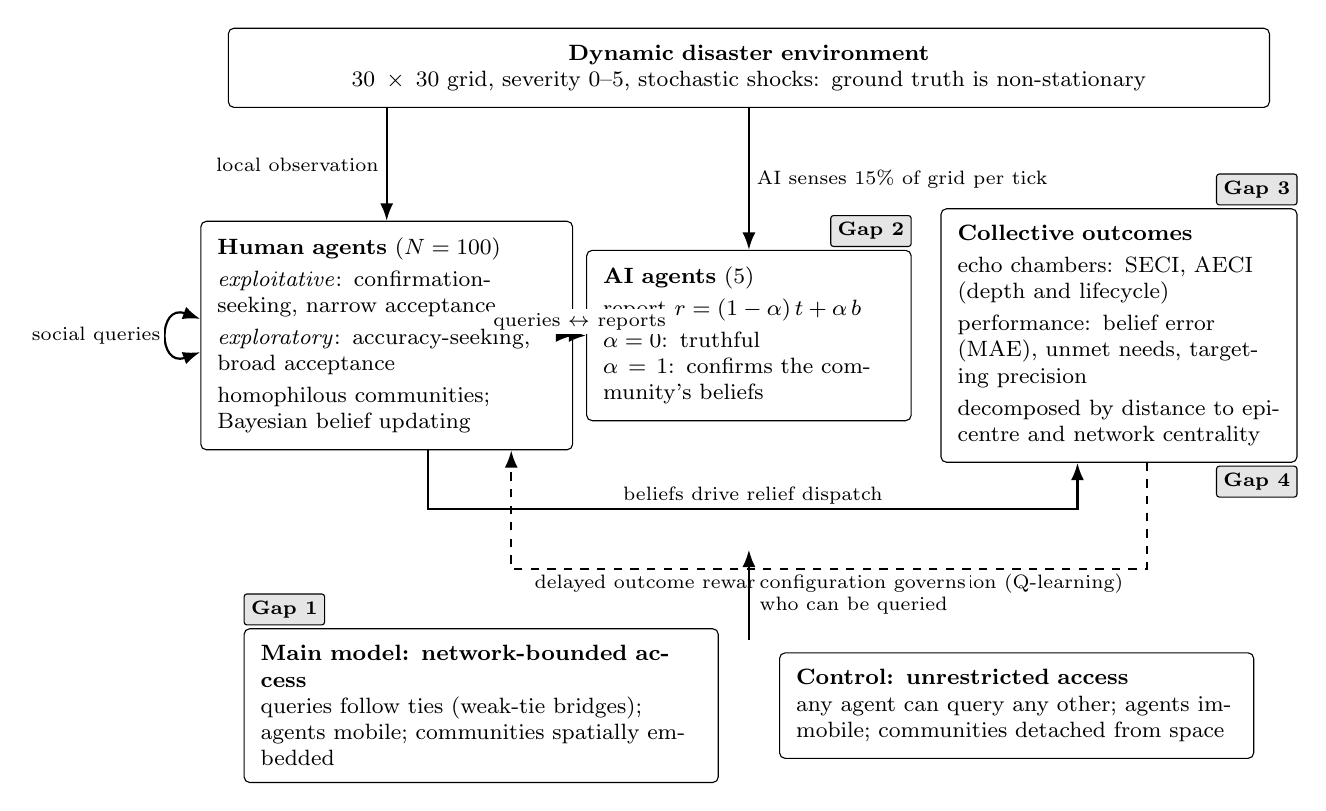
\begin{tikzpicture}[
  font=\footnotesize,
  box/.style={draw, rounded corners=2pt, align=left, inner sep=6pt},
  gapbadge/.style={draw, rounded corners=1pt, fill=black!10, inner sep=2.5pt, font=\scriptsize\bfseries},
  lab/.style={font=\scriptsize, fill=white, inner sep=1.5pt},
  arr/.style={-{Latex[length=2.2mm]}, thick},
  arrd/.style={-{Latex[length=2.2mm]}, thick, dashed},
  biarr/.style={{Latex[length=2.2mm]}-{Latex[length=2.2mm]}, thick}
]
% ---------- Environment ----------
\node[box, align=center, text width=12.8cm] (env) at (7.0,0)
  {\textbf{Dynamic disaster environment}\\
   $30 \times 30$ grid, severity 0--5, stochastic shocks: ground truth is non-stationary};

% ---------- Actors and outcomes ----------
\node[box, text width=4.3cm] (hum) at (2.4,-3.4)
  {\textbf{Human agents} ($N = 100$)\\[2pt]
   \emph{exploitative}: confirmation-seeking, narrow acceptance\\[2pt]
   \emph{exploratory}: accuracy-seeking, broad acceptance\\[2pt]
   homophilous communities;\\ Bayesian belief updating};
\node[box, text width=3.7cm] (ai) at (7.0,-3.4)
  {\textbf{AI agents} (5)\\[2pt]
   report $r = (1-\alpha)\,t + \alpha\,b$\\[2pt]
   $\alpha = 0$: truthful\\
   $\alpha = 1$: confirms the community's beliefs};
\node[box, text width=4.1cm] (out) at (11.7,-3.4)
  {\textbf{Collective outcomes}\\[2pt]
   echo chambers: SECI, AECI (depth and lifecycle)\\[2pt]
   performance: belief error (MAE), unmet needs, targeting precision\\[2pt]
   decomposed by distance to epicentre and network centrality};

% ---------- Environment to actors ----------
\draw[arr] (env.south -| hum.north) -- node[lab, left=1pt]{local observation} (hum.north);
\draw[arr] (env.south -| ai.north)  -- node[lab, right=1pt]{AI senses 15\% of grid per tick} (ai.north);

% ---------- Query channels ----------
\draw[biarr] (hum.east |- ai.west) -- node[lab, above]{queries $\leftrightarrow$ reports} (ai.west);
\draw[biarr] ([yshift=6pt]hum.west) to[out=160, in=200, looseness=3.5]
  node[lab, left=1pt]{social queries} ([yshift=-6pt]hum.west);

% ---------- Beliefs to decisions and feedback ----------
\coordinate (fwd1) at ([xshift=15pt]hum.south);
\coordinate (fwd2) at ([xshift=-15pt]out.south);
\draw[arr]  (fwd1) -- ++(0,-0.75) -| node[lab, above, pos=0.25]{beliefs drive relief dispatch} (fwd2);
\coordinate (fb1) at ([xshift=-15pt]out.south west |- out.south);
\coordinate (fb2) at ([xshift=45pt]hum.south);
\draw[arrd] ([xshift=25pt]fwd2) -- ++(0,-1.35) -|
  node[lab, below, pos=0.25]{delayed outcome rewards shape source selection (Q-learning)} (fb2);

% ---------- Configurations ----------
\node[box, text width=5.6cm] (main) at (3.6,-8.1)
  {\textbf{Main model: network-bounded access}\\ queries follow ties (weak-tie bridges); agents mobile; communities spatially embedded};
\node[box, text width=5.6cm] (ctrl) at (10.4,-8.1)
  {\textbf{Control: unrestricted access}\\ any agent can query any other; agents immobile; communities detached from space};
\coordinate (cmid) at ($(main.north east)!0.5!(ctrl.north west)$);
\draw[arr] (cmid) -- node[lab, right=2pt, align=left]{configuration governs\\ who can be queried} ++(0,1.15);

% ---------- Gap badges ----------
\node[gapbadge, anchor=south west] at ([yshift=1pt]main.north west) {Gap 1};
\node[gapbadge, anchor=south east] at ([yshift=1pt]ai.north east)   {Gap 2};
\node[gapbadge, anchor=south east] at ([yshift=1pt]out.north east)  {Gap 3};
\node[gapbadge, anchor=north east] at ([yshift=-1pt]out.south east) {Gap 4};
\end{tikzpicture}}
\caption{Conceptual overview of the model and its mapping to the research gaps. A non-stationary disaster environment is observed locally by 100 human agents of two cognitive types and partially sensed by five AI agents. Humans query their social contacts or the AI, whose reports interpolate between truth and confirmation via the alignment parameter $\alpha$ (Gap~2). Beliefs drive relief decisions whose delayed outcomes feed back into source selection. Which contacts can be queried is governed by the configuration: the main model bounds access by a spatially embedded social network with mobility, the control leaves access unrestricted (Gap~1). Outcomes are measured at the level of communities and the population (Gap~3) and decomposed by position in space and network (Gap~4). Parameters in Supplementary Table~S1.}\label{fig:concept}
\end{figure}

\section{Results}\label{sec:results}

Throughout, the alignment parameter is swept over eleven levels ($\alpha = 0.0, 0.1, \ldots, 1.0$) with $N = 20$ replications per level, and every sweep is run under both configurations of Fig.~\ref{fig:concept} on identical random seeds, so that the two can be compared replicate by replicate; steady-state values are means over the last 75 of 200 ticks. Table~\ref{tab:metrics} summarises the outcome metrics (formal definitions in the Methods, Sec.~\ref{sec:metrics}). Echo chambers are, at their core, a loss of belief diversity. The Social Echo Chamber Index (SECI) compares the belief variance within each social community to that of the whole population, restricted to disaster-affected cells; the AI Echo Chamber Index (AECI-Var) applies the identical comparison but groups agents by their reliance on the AI, so that negative values mark a bubble of AI-reliant users converging on shared beliefs regardless of their social position. Because variance-based indices cannot distinguish convergence on the truth from convergence on a shared error, they are always read together with two accuracy measures -- AECI-Err, negative when AI-reliant agents are more \emph{confidently wrong} than AI-light agents, and the belief error (MAE) over affected cells -- and with two operational metrics, \emph{unmet needs} and \emph{targeting precision}.

\begin{table}[h]
\caption{Outcome metrics used throughout the Results. Formal definitions and design rationale in the Methods (Sec.~\ref{sec:metrics}).}\label{tab:metrics}
\footnotesize
\begin{tabular}{@{}lp{6.6cm}l@{}}
\toprule
Metric & What it captures & Reading \\
\midrule
SECI & Belief homogeneity within social communities relative to the population (affected cells only) & $<0$: social echo chamber \\
AECI-Var & Belief homogeneity among the most AI-reliant agents relative to the population & $<0$: AI-induced bubble \\
AECI-Err & Confidence-weighted belief error of AI-reliant vs.\ AI-light agents & $<0$: AI users confidently wrong \\
Belief MAE & Mean absolute belief error over affected cells & lower is better \\
Unmet needs & High-need cells (severity $\geq 3$) receiving no relief per tick & lower is better \\
Precision & Share of relief tokens placed on high-need cells & higher is better \\
\botrule
\end{tabular}
\end{table}

\subsection{Network-bounded access is a precondition for AI-amplified echo chambers}\label{sec:claim1}

The two configurations produce opposite trends at high alignment (Fig.~\ref{fig:comparison}; paired per-seed differences in Supplementary Table~S11, where replicate $i$ uses the same seed in both configurations, so a confidence interval excluding zero marks an effect robust across disaster realisations). In the control, the social echo chamber attenuates with alignment: SECI rises from $-0.256 \pm 0.024$ at $\alpha = 0$ to $-0.140 \pm 0.038$ at $\alpha = 1$ (mean $\pm$ s.e.m., $N = 20$). The main model tracks the control closely for $\alpha \leq 0.6$ and then departs from it: from $\alpha = 0.7$ the paired $\Delta$SECI becomes negative and seed-robust ($-0.068$, 95\% CI $[-0.110, -0.026]$), growing to $-0.192$ $[-0.257, -0.127]$ at $\alpha = 0.9$, where the main model reaches SECI $= -0.329 \pm 0.051$. Community-level belief convergence thus weakens with confirmation when access is unrestricted and deepens sharply when access follows network ties. The AI-side index behaves differently: AECI-Var attenuates with alignment in both configurations (from $-0.279 \pm 0.028$ and $-0.240 \pm 0.024$ at $\alpha = 0$ to $-0.166 \pm 0.028$ and $-0.163 \pm 0.037$ at $\alpha = 1$), and AECI-Err remains close to zero up to $\alpha = 0.8$, turning positive at $\alpha \geq 0.9$ -- consistent with degraded beliefs becoming pervasive across the population rather than concentrated among AI users.

\begin{figure}[h]
\centering

\includegraphics[width=\textwidth]{comparison_configs.png}
\caption{Configuration comparison across the primary alignment sweep (raw metrics; mean $\pm$ s.e.m. over $N=20$ paired replications). Top row: SECI, AECI-Var and AECI-Err; for all three, negative values indicate an echo chamber. Bottom row: belief MAE over affected cells, unmet high-need cells per tick, and relief targeting precision. Blue: control (global access, immobile agents, disconnected communities); orange: main model (network-gated access, mobility, spatially embedded bridged network). Paired per-seed differences in Supplementary Table~S11.}\label{fig:comparison}
\end{figure}

Together, these patterns identify network-bounded access as a structural precondition for AI amplification of social echo chambers. The mechanism follows from the model's confirmation targeting: for exploitative queriers, a confirming AI targets the consensus belief of the caller's trusted network. Under unrestricted access, roughly half of human queries reach agents outside the caller's community, so out-group beliefs continuously perturb community consensus and the confirming signal cannot compound. Under network-gated access, communities are epistemically closed except for sparse weak-tie bridges, and a consensus-targeting AI recycles each community's shared belief back into it, deepening within-community convergence precisely at high alignment. That the strongly negative variance indices at $\alpha = 0$ do not signal comparable harm is confirmed by the accuracy metrics: at low alignment, homogeneity coincides with low belief error (Fig.~\ref{fig:comparison}, bottom left), so convergence is convergence on the truth, whereas the deepening SECI at high alignment coincides with the largest belief errors of the sweep.

\subsection{A truthful AI builds a bubble of its own: the alignment optimum is interior only under network-bounded access}\label{sec:claim2}

A fully truthful AI is not automatically the safest choice: it creates an echo chamber of its own. Across the main-model sweep, AECI-Var is strongest at the truthful end ($-0.25$ at $\alpha \leq 0.1$) and weakest at $\alpha = 0.8$ ($-0.112$) -- the agents who rely most on the shared source converge tightly on its estimates, regardless of their social ties (Fig.~\ref{fig:goldilocks}). The social chamber moves in the opposite direction: SECI remains between $-0.20$ and $-0.24$ for $\alpha \leq 0.8$ and deepens to $-0.30$ to $-0.33$ at $\alpha \geq 0.9$. Because the two chamber mechanisms penalise opposite ends of the alignment axis, their normalised sum -- the bubble-only composite -- is minimised in the interior, at $\alpha^{*} = 0.8$, with a nearly as deep local minimum at $\alpha = 0.5$; adding the normalised belief error, which grows beyond $\alpha \approx 0.4$, shifts the minimum to $\alpha^{*}(+\text{MAE}) = 0.5$, with near-minima at 0.3 and 0.4. The optimum is interior on the operational side as well: unmet high-need cells reach their minimum in the mid-range (0.33 cells per tick at $\alpha = 0.5$, against 1.17 at $\alpha = 0$) while targeting precision stays flat near 0.78 up to $\alpha = 0.7$ before declining.

\begin{figure}[h]
\centering
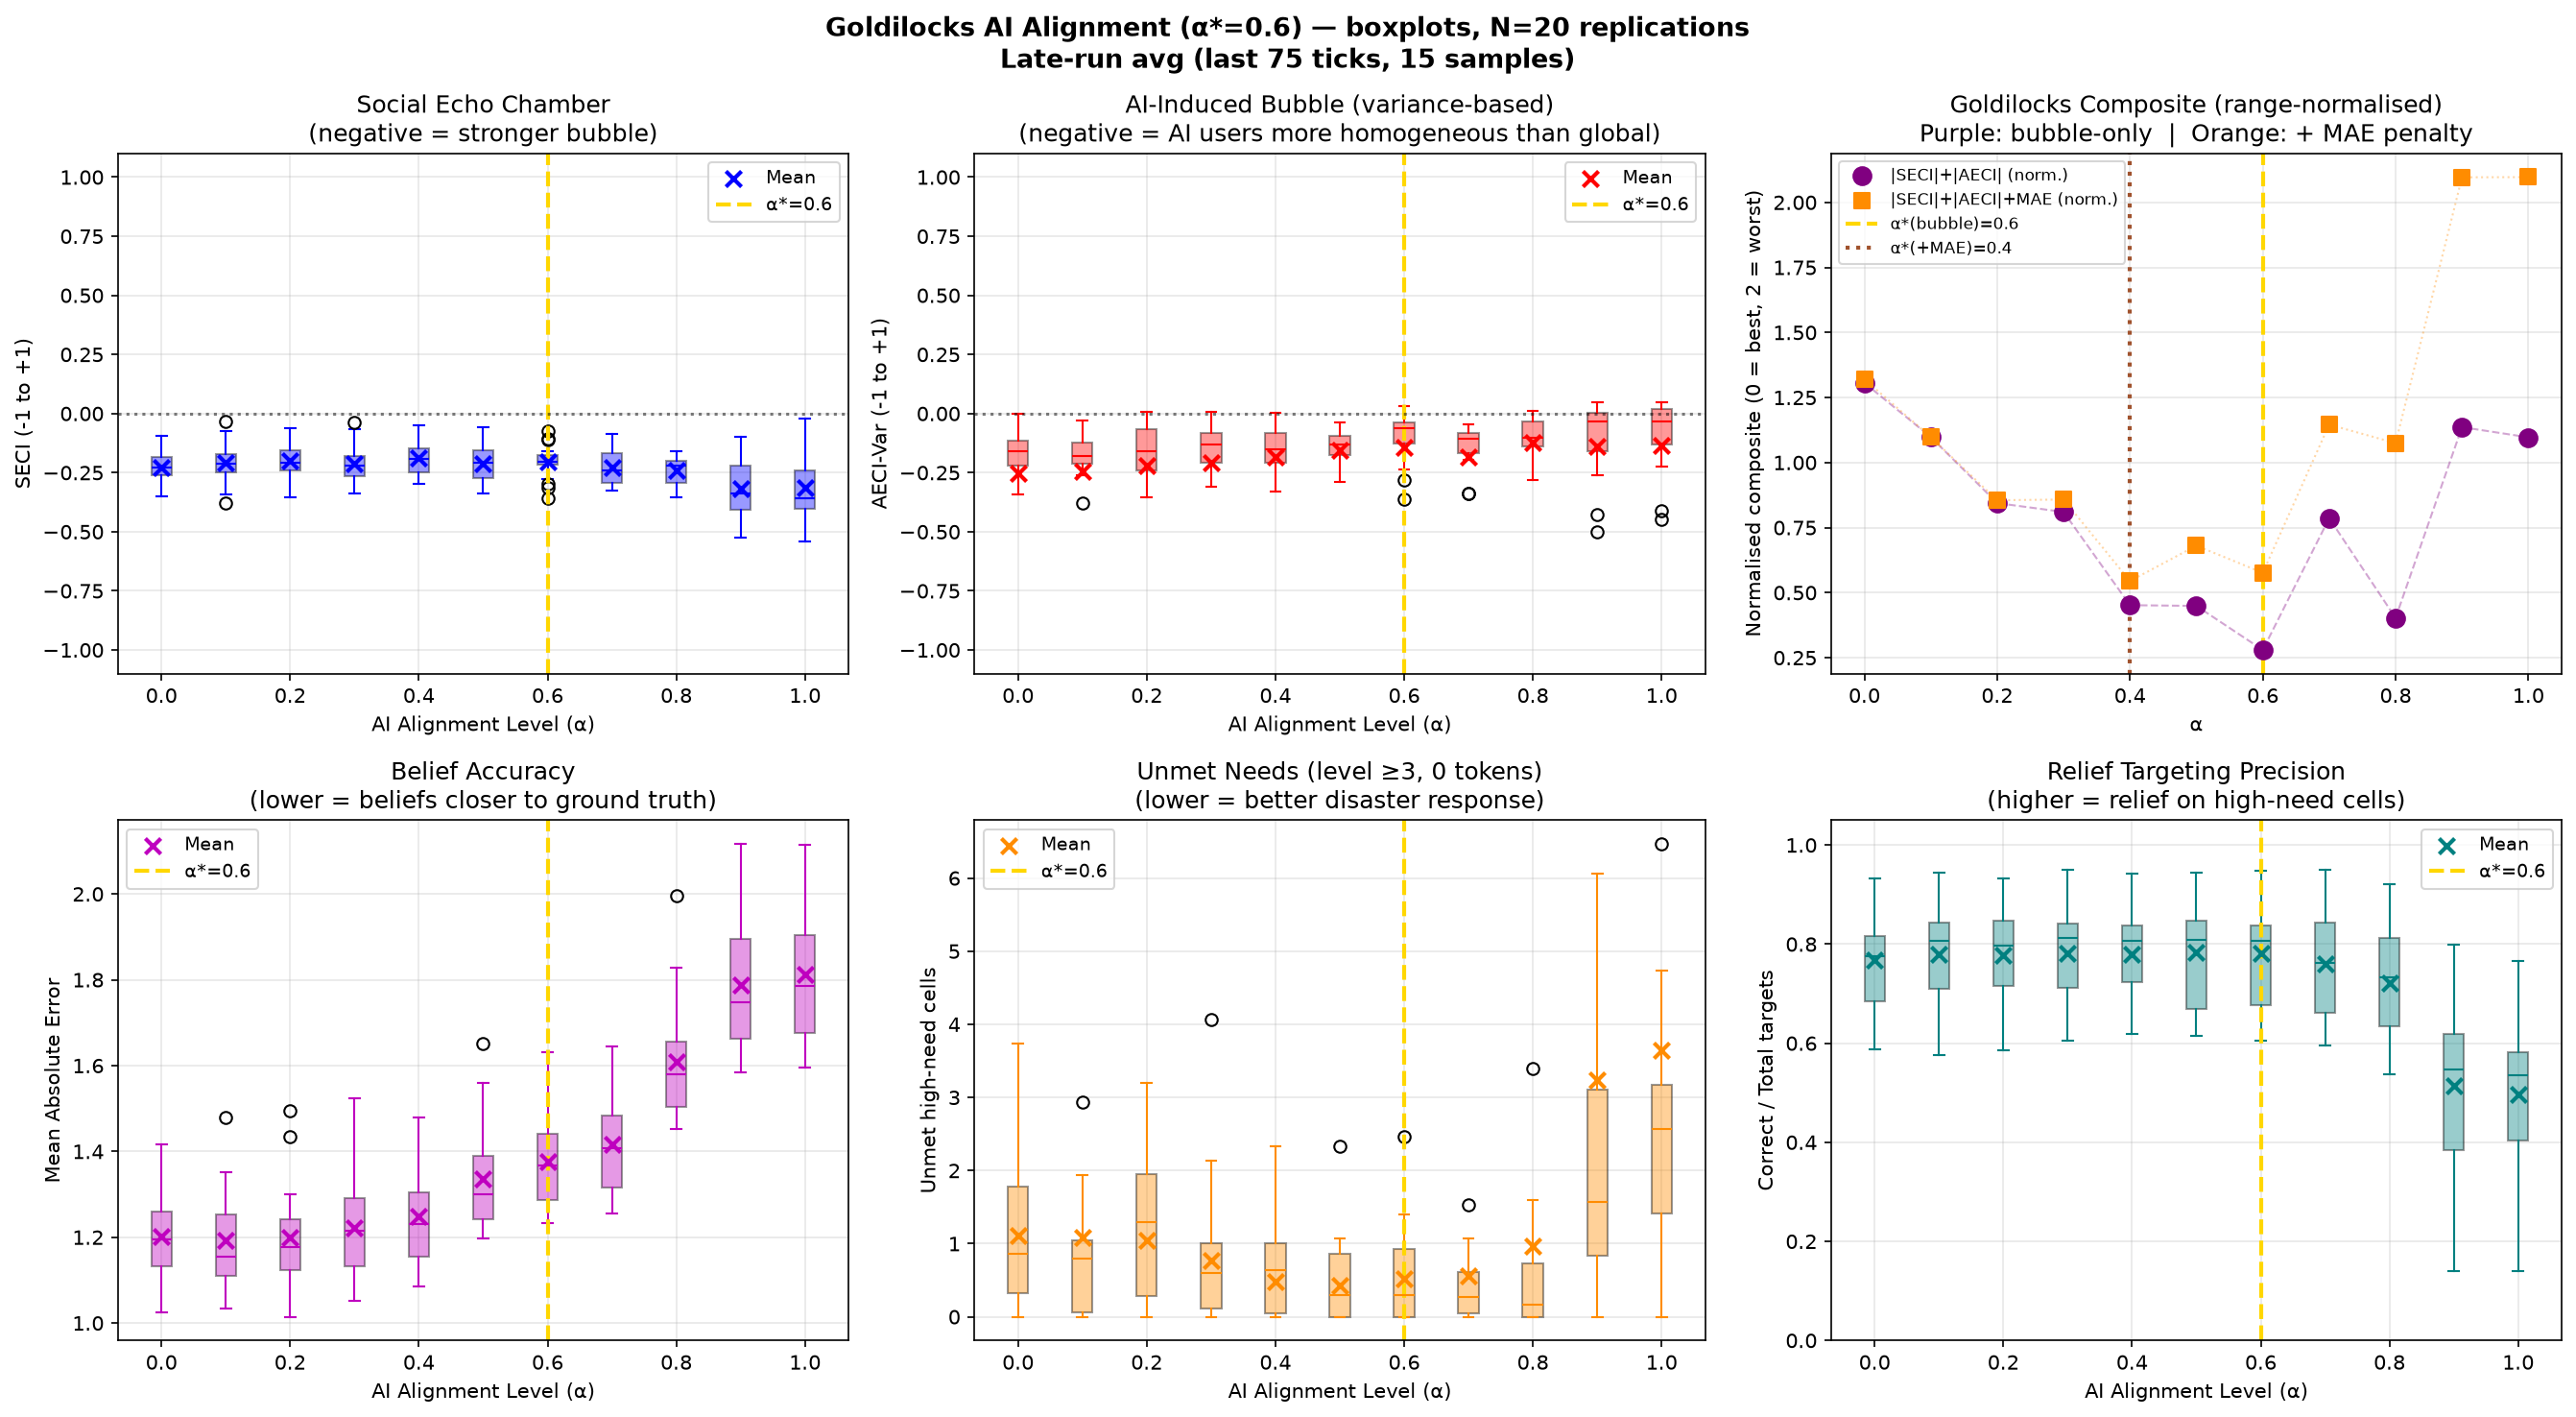
\includegraphics[width=\textwidth]{goldilocks_alignment_sweep.png}
\caption{Alignment sweep under the main model ($N=20$ replications per level; steady state, last 75 ticks). Boxplots show medians, interquartile ranges and 1.5$\times$IQR whiskers; crosses mark means. The composite panel (top right) shows the range-normalised bubble-only composite $|\text{SECI}|_{\text{norm}} + |\text{AECI-Var}|_{\text{norm}}$ (purple) and the operational composite including normalised MAE (orange). Dashed and dotted vertical lines mark $\alpha^{*}(\text{bubble}) = 0.8$ and $\alpha^{*}(+\text{MAE}) = 0.5$.}\label{fig:goldilocks}
\end{figure}

Because range normalisation can amplify a component with a small raw signal, we treat the \emph{interiority} of $\alpha^{*}$ -- not its exact location -- as the property that must survive scrutiny. Under the main model, all six composite variants (SECI alone, SECI + AECI-Var, SECI + AECI-Err, each with and without the MAE penalty) place the optimum strictly in the interior; under the control, the bubble composites are minimised at or next to the boundary, $\alpha^{*} \in \{0.9, 1.0\}$ (Supplementary Fig.~S6). Paired per-seed contrasts of the \emph{raw} composite confirm this is no normalisation artefact: in the main model every interior level $\alpha \in [0.3, 0.8]$ beats the truthful endpoint (e.g., $-0.102$ $[-0.166, -0.038]$ at $\alpha = 0.5$) and $\alpha = 0.8$ beats the confirming endpoint ($-0.116$ $[-0.213, -0.020]$), whereas in the control the mid-range is significantly \emph{worse} than full confirmation ($+0.169$ $[+0.044, +0.295]$ at $\alpha = 0.5$). Decomposition attributes the truthful endpoint's penalty almost entirely to AECI-Var -- the shared-source bubble -- and the confirming endpoint's almost entirely to SECI -- consensus recycling; since the latter mechanism operates only under network-bounded access (Sec.~\ref{sec:claim1}), interiority itself is a structural property. Between the endpoints the objective is statistically flat, so only ranges carry information: echo-chamber suppression favours $\alpha^{*} \approx 0.4$--$0.8$, the operational composites $\alpha^{*} \approx 0.3$--$0.5$.

Whether an interior optimum exists at all is moreover a property of the population's cognitive profile, swept in a separate batch of 2{,}640 runs over the cognitive gap $g$ between the two agent types and the acceptance midpoint $d_{\text{mid}}$ (Fig.~\ref{fig:gapsweep}; Methods, Supplementary S7). In cognitively homogeneous populations ($g = 0$) with baseline or open acceptance, the optimum is $\alpha^{*} = 0$: a fully truthful AI. The interior optimum emerges once confirmation-seeking agents are present ($g \geq 0.5$), or when the entire population is closed-minded ($d_{\text{mid}} = 2.0$, where $\alpha^{*} = 0.7$ even at $g = 0$), and $\alpha^{*}$ rises with both polarisation and closedness, saturating at 0.8, while open populations keep it at 0.3--0.4. The cost paid \emph{at the optimum} rises along both axes as well -- belief error at $\alpha^{*}$ grows from 1.12 (open, homogeneous) to 1.63 (closed, polarised) -- so populations that require more confirmation to accept information are worse off even under their own optimal policy.

\begin{figure}[h]
\centering

\includegraphics[width=\textwidth]{gap_sweep.png}
\caption{The alignment optimum as a function of the population's cognitive profile ($4 \times 3 \times 11$ conditions, $N = 20$ replications each, main-model configuration). Top left: $\alpha^{*}$ under the bubble-only (solid) and bubble+MAE (dashed) criteria across the cognitive gap $g$, for closed ($d_{\text{mid}} = 2.0$), baseline (3.0) and open (4.0) acceptance midpoints. Top right: raw bubble composite at $\alpha^{*}$. Bottom: SECI and belief error at $\alpha^{*}$. Full grid in Supplementary Table~S7b.}\label{fig:gapsweep}
\end{figure}

The temporal dynamics argue for the lower half of the interior range. Peak chamber strength varies little with alignment, but recovery is strongly alignment-dependent (Fig.~\ref{fig:lifecycle}): exploitative chambers recover by ticks 40--55 for $\alpha \leq 0.8$ and never recover at $\alpha \geq 0.9$; exploratory chambers recover progressively later as alignment grows and fail to recover at all for $\alpha \geq 0.7$, with the fraction of the run spent inside a chamber rising from roughly 0.4--0.6 in the low-to-mid range to 0.70--0.85 at high alignment. The operational optima ($\alpha \approx 0.3$--$0.5$) thus coincide with the highest alignment levels at which chambers still dissolve within the response horizon, whereas the bubble composite's minimum at $\alpha = 0.8$ lies in a regime where exploratory chambers no longer recover. The query behaviour behind this collapse completes the picture: a confirming AI progressively captures the queries of precisely the confirmation-seeking agents it is tuned to satisfy (steady-state AI share rising from 0.39 at $\alpha = 0$ to 0.58 at $\alpha = 1$), while exploratory agents' reliance is stable at 0.50--0.59 -- their vulnerability arises through the silent failure of verification-based correction, not through increased querying (Supplementary Fig.~S7; full time series in Supplementary Figs.~S1--S2).

\begin{figure}[h]
\centering
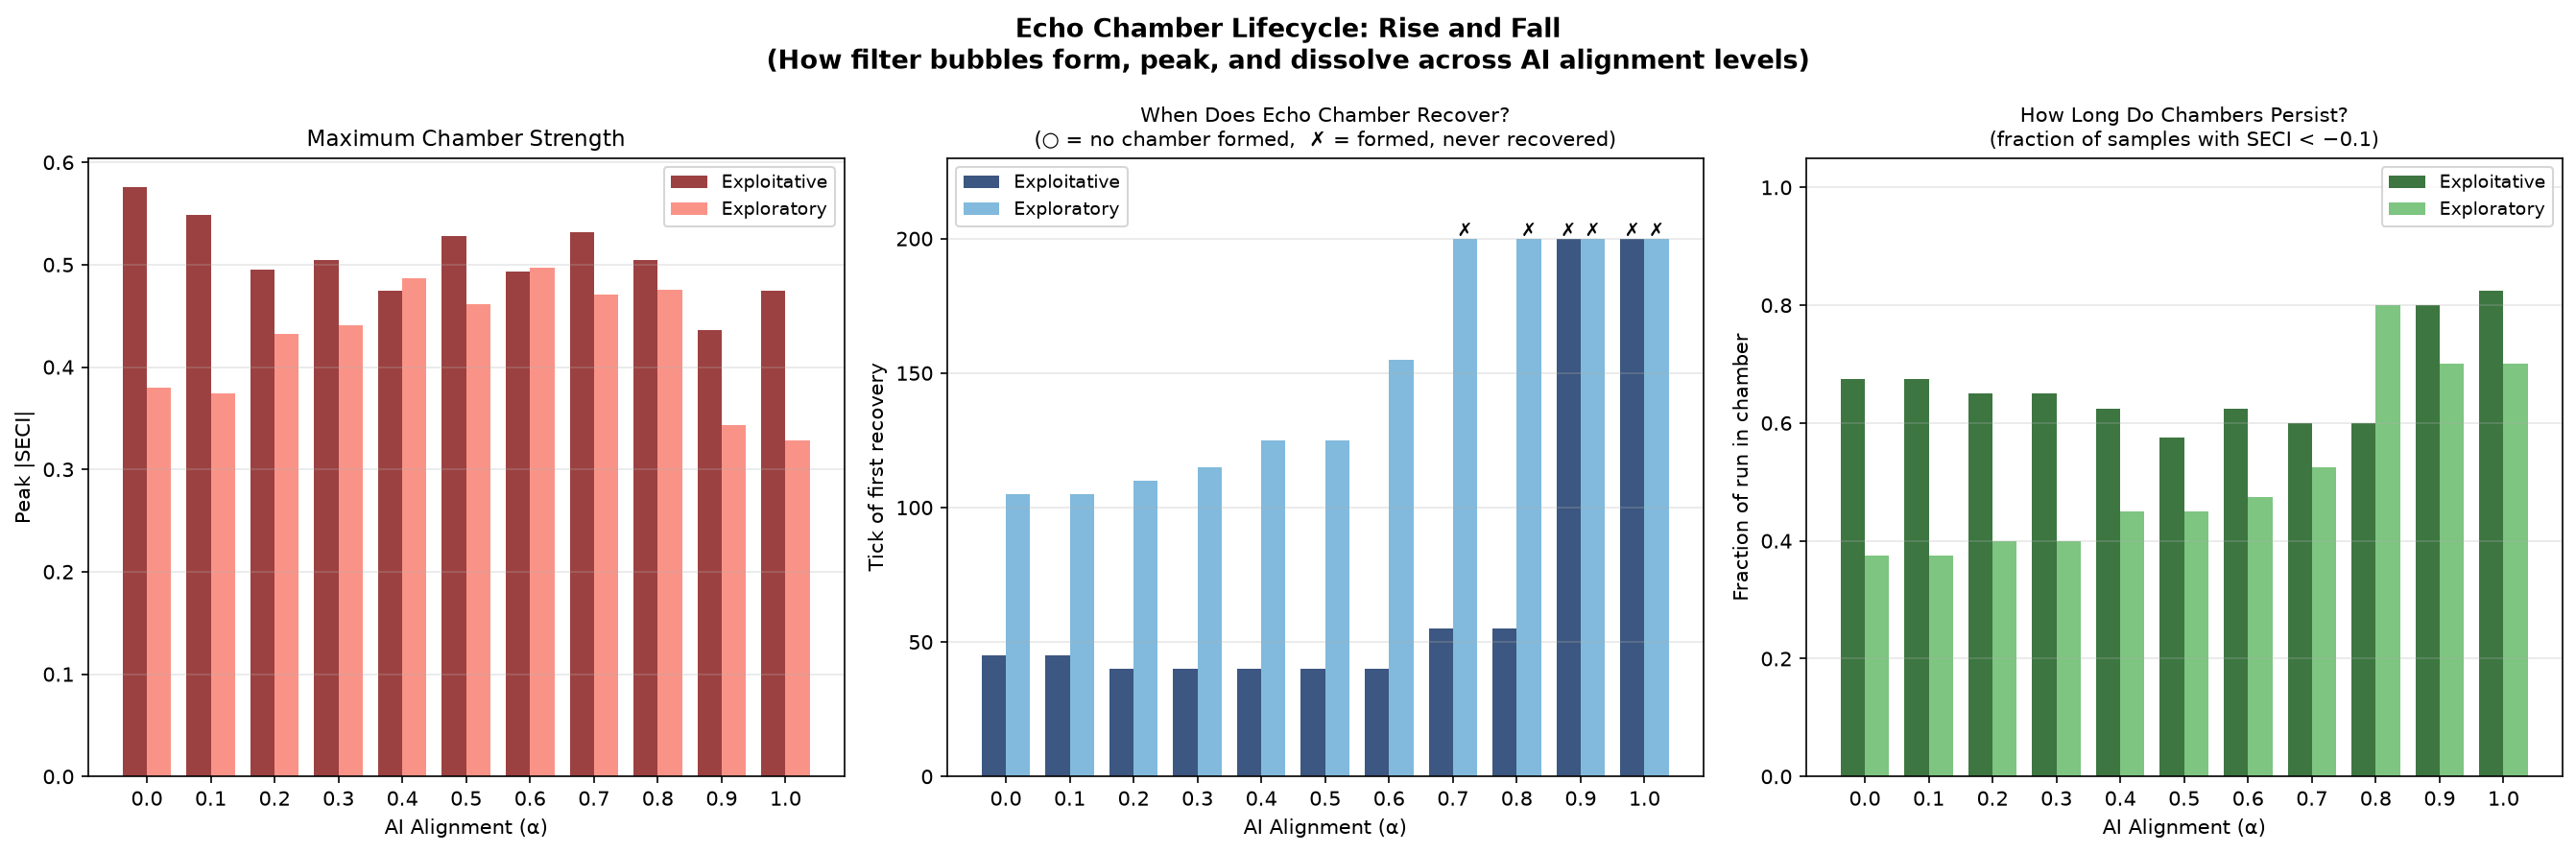
\includegraphics[width=\textwidth]{echo_chamber_lifecycle.png}
\caption{Echo chamber lifecycle across alignment levels in the main model, by agent type. Left: maximum chamber strength (peak $|\text{SECI}|$). Middle: tick of first recovery, defined as SECI sustained above $-0.05$ for three consecutive samples after having formed below $-0.1$; crosses mark conditions in which chambers never recover within the 200-tick run. Right: fraction of the run spent inside a chamber (SECI $< -0.1$).}\label{fig:lifecycle}
\end{figure}

\subsection{The belief--decision--feedback loop buffers operational collapse under network-bounded access}\label{sec:claim3}

Echo chambers matter beyond the belief state itself: agents act on their beliefs by dispatching relief, outcomes return as delayed rewards, and Q-learning translates those rewards into future source selection, so the loop determines whether chambers correct or entrench (Gap~3). On all three decision-side metrics, the structural constraints that expose communities to consensus recycling simultaneously improve operational performance across the entire sweep. Belief MAE is lower in the main model at every alignment level, with seed-robust paired differences ranging from $-0.082$ $[-0.119, -0.044]$ at $\alpha = 0$ to $-0.166$ $[-0.211, -0.121]$ at $\alpha = 1$, and targeting precision shows the mirror image, rising from about $+0.06$--$0.10$ over most of the sweep to $+0.318$ $[+0.218, +0.418]$ at $\alpha = 0.9$ (Fig.~\ref{fig:comparison}, bottom row; Supplementary Table~S11). The clearest contrast concerns the collapse of relief delivery under near-full confirmation: in the control, unmet high-need cells jump from $2.3 \pm 0.3$ at $\alpha = 0.8$ to $11.3 \pm 0.5$ at $\alpha = 0.9$ while precision falls from 0.63 to 0.21, whereas the main model degrades far less severely (unmet needs $3.1 \pm 0.5$, precision 0.53) -- paired deltas of $-8.2$ $[-9.7, -6.8]$ unmet cells per tick, a reduction of the collapse by more than a factor of three. The degradation that remains is slower but real: at high alignment, unmet needs decline substantially more slowly over the run -- which matters because deprivation costs accumulate with the time needs remain unmet \citep{holguin2012unique} -- and the relief effort both shrinks (from 401 to 331 tokens per tick across the sweep) and concentrates its shortfall on the worst-served cells (Supplementary Figs.~S1 and~S3).

Two mechanisms drive this robustness, and both operate independently of the AI. Mobility gives agents genuine direct-observation coverage, so a fraction of every community's information is grounded in first-hand sensing that no degree of AI confirmation can distort; network-gated querying concentrates exchange on trusted contacts whose local observations are, on average, accurate about the caller's surroundings. Because part of every agent's reward signal is thereby grounded in observation and trusted local reports, source-selection learning keeps receiving corrective evidence even when the AI confirms. The comparison between configurations thus reveals a trade-off rather than a uniform benefit of structural realism: the same network boundedness that anchors operational performance is what allows a highly aligned AI to deepen social echo chambers (Sec.~\ref{sec:claim1}). Structural realism shifts the failure mode of sycophantic AI from operational collapse towards epistemic insularity.

\subsection{Harms of alignment concentrate on the spatial periphery}\label{sec:claim4}

The first three findings operate at the level of the population; the fourth traces how the harm is distributed within it (Gap~4). The belief-error gap between agents spawned far from and near to the epicentre widens monotonically with alignment, from $+0.15$ at $\alpha = 0$ to $+0.37$ at $\alpha = 1$ (Fig.~\ref{fig:periphery}): agents remote from the events, who depend almost entirely on mediated reports, absorb most of the accuracy loss that confirmation produces. The behavioural consequence is withdrawal from the response: relief contributed by far-spawned agents falls from 16.2 to 6.2 tokens per agent per five-tick window across the sweep ($-62\%$), while near-spawned agents reduce their contribution far less (18.5 to 13.4, $-28\%$) -- the remote quartile does not merely become less accurate, it largely stops sending assistance. Network position offers no comparable protection: the belief-error difference between high- and low-centrality agents stays within 0.06 at every alignment level. The harms of a confirming AI are thus spatially, not topologically, structured: they fall on those who cannot verify reports against first-hand observation, regardless of how well connected they are -- precisely the position of the remote coordination hubs that dominate data-driven crisis response \citep{comes2020coordination,coleman2024weaving}. The cognitive-gap and factor sweeps (Supplementary S7--S8) probe how far the findings extend: the interior optimum requires confirmation-seeking agents or a uniformly closed population (S7), and early relief failure traces to rumour prevalence and exploitative composition rather than hazard tempo (S8).

\begin{figure}[h]
\centering
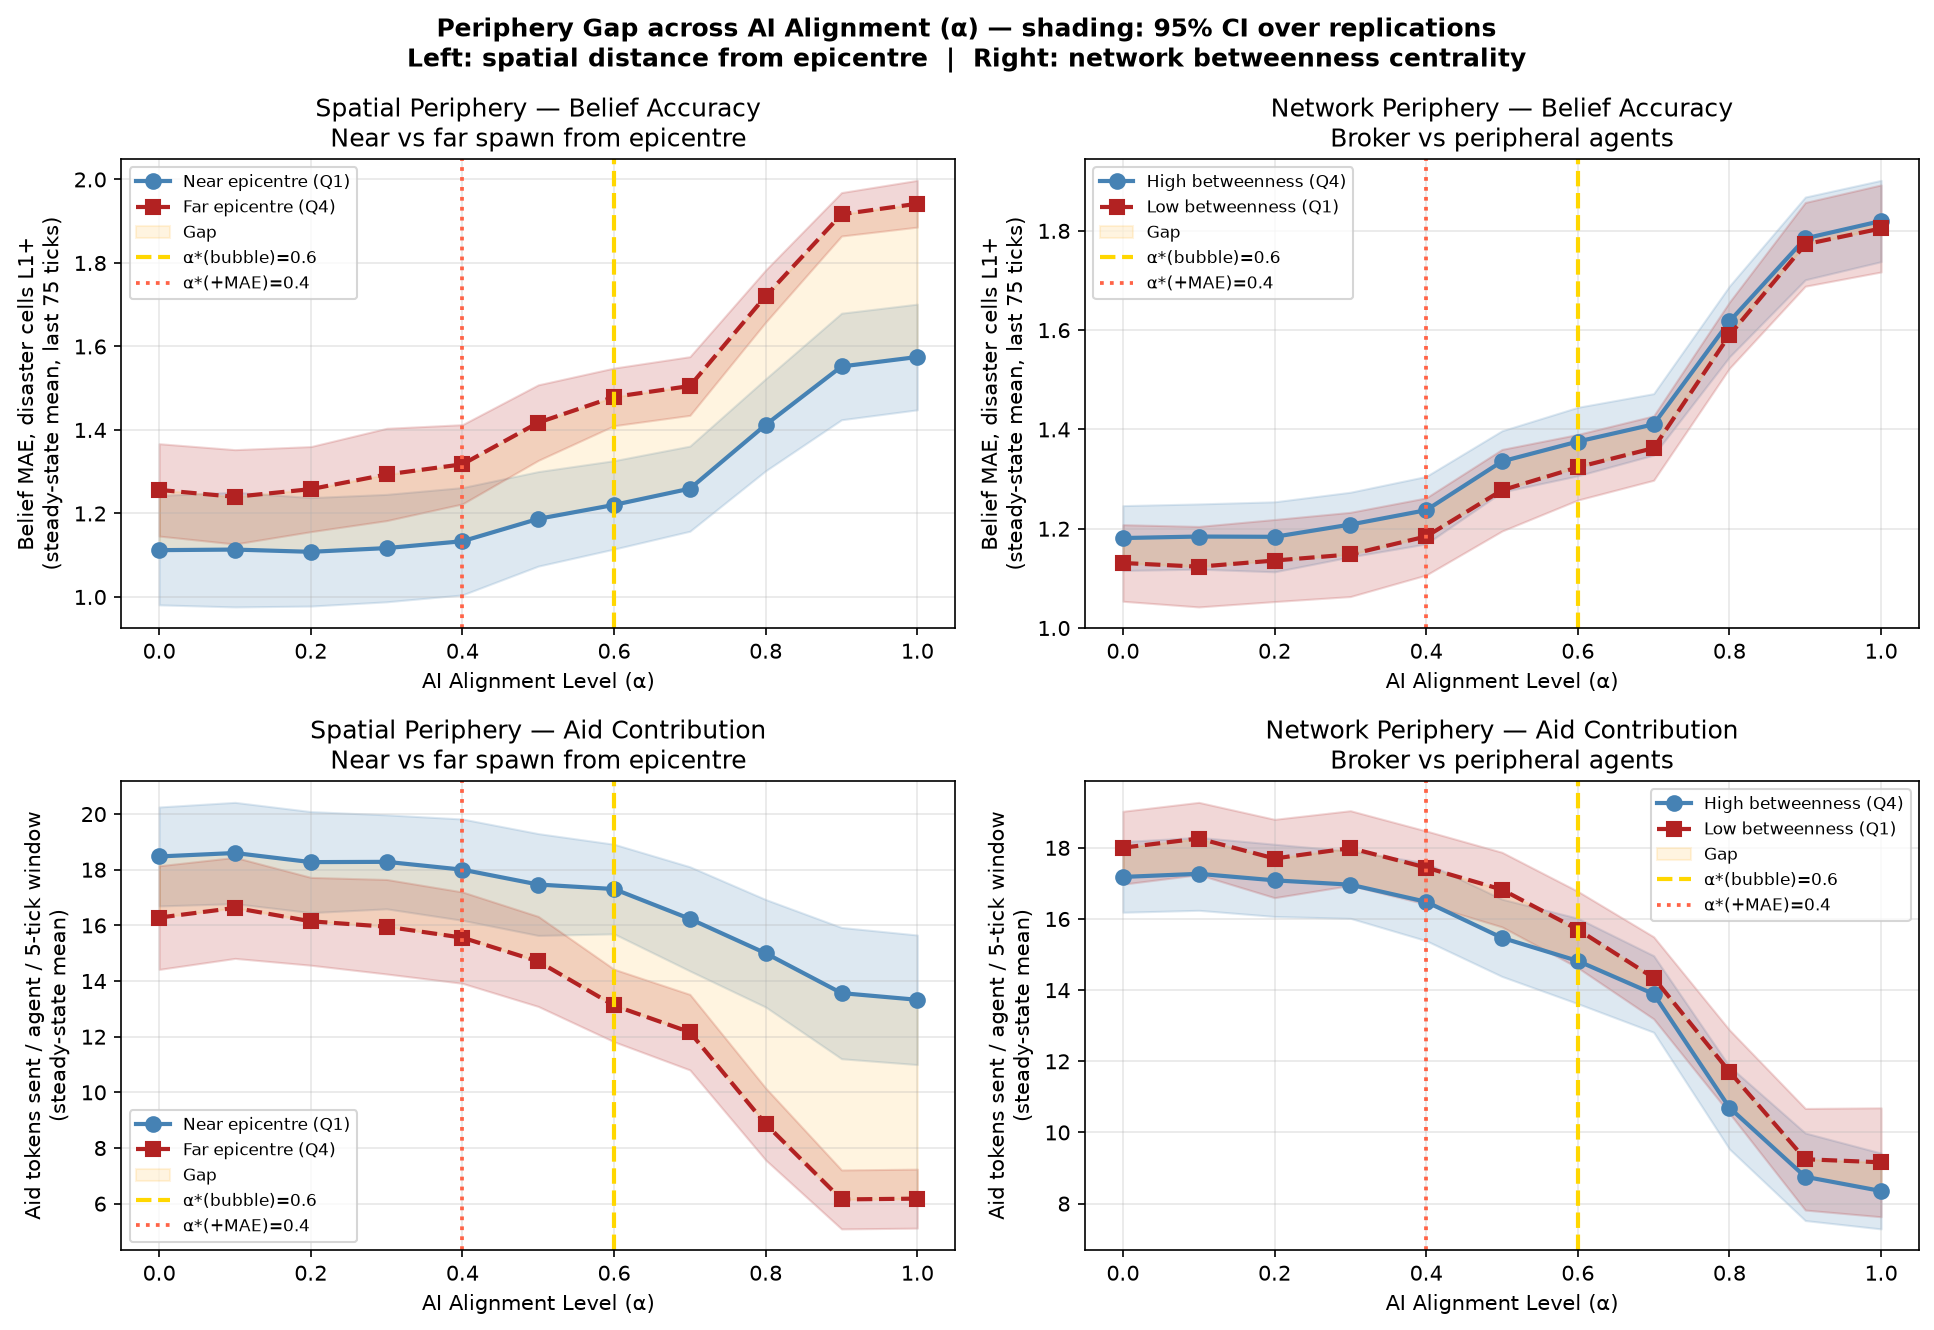
\includegraphics[width=\textwidth]{periphery_gap.png}
\caption{Distribution of alignment harms across space and the social network (main model; steady state, last 75 ticks; $N = 20$). Top: belief error and relief contribution by distance of the agent's home location to the epicentre (nearest vs.\ furthest quartile). Bottom: the same decomposition by betweenness centrality (top vs.\ bottom quartile). Bands show 95\% confidence intervals across replications.}\label{fig:periphery}
\end{figure}

\section{Discussion}\label{sec:discussion}

This paper asked whether an AI trained to please its users breaks echo chambers or reinforces them -- and at what cost to the decisions that depend on the resulting beliefs. The answer is conditional: the direction of AI influence on collective belief structure depends on whether information access is bounded by network structure and space. Under unrestricted access, a belief-confirming AI degrades accuracy and relief performance without deepening community-level convergence; under network-bounded access, the same AI drives communities into progressively deeper and, beyond $\alpha \approx 0.7$, unrecoverable echo chambers. Four implications follow, one per gap.

First (Gap~1), the results extend the experimental literature on human--AI feedback loops from dyads to networks. Interaction with biased AI amplifies individual biases beyond what human--human interaction produces \citep{glickman2024human}; whether that amplification aggregates into collective echo chambers is governed by a variable invisible at the dyadic level -- the structure of who can query whom -- paralleling results in networked collective intelligence, where the effect of social influence on crowd accuracy reverses with network structure \citep{lorenz2011social,becker2017network}. The control shows what a stylised model without structural constraints would have concluded: that confirmation weakens echo chambers, with an optimal alignment of 1.0 on bubble criteria. This null result is an artefact of unrestricted access, and it suggests that models omitting network-bounded access systematically underestimate the epistemic risks of belief-aligned AI while overestimating its operational risks. Collective epistemic risk assessments of AI require network-level analysis.

Second (Gap~2), the alignment paradox \citep{west2025alignment} acquires a structural qualification. The paradox holds -- AI tuned to confirm community beliefs produces exactly the insularity it is meant to overcome -- yet only where the social fabric channels information along ties. At the same time, a fully truthful AI is not the remedy it appears to be: its reports concentrate its heaviest users around a shared estimate, an AI echo chamber that forms regardless of social ties. Both extremes are dominated by moderate alignment, and where a criterion places its optimum follows from which mechanism it penalises: accuracy-sensitive criteria push $\alpha^{*}$ towards the truthful end, variance-based criteria tolerate higher alignment, and the recovery dynamics cap acceptable alignment at $\alpha \approx 0.7$. The operational range $\alpha^{*} \approx 0.3$--$0.5$ is where these demands overlap -- with the caveat that variance-based indices must always be read jointly with belief accuracy, since they cannot distinguish convergence on truth from convergence on error. Taken together with Gap~1, the dose--response curve of alignment has a different shape in differently structured populations: the identical AI policy is benign, optimal or harmful depending on the population it serves.

Third (Gap~3), the belief--decision--feedback loop reframes what should be monitored when belief-aligned AI is deployed. Because part of every agent's reward signal remains grounded in first-hand observation and trusted local reports, operational performance degrades gradually even as confirmation rises -- and precisely this graceful degradation is the risk: belief error and relief precision would appear manageable in operational dashboards even while social echo chambers deepen past the point of recovery. Monitoring should therefore target community-level belief convergence in addition to individual accuracy and aggregate performance. The timing results sharpen the concern: recovery collapses first among the accuracy-seeking exploratory agents -- precisely those whom conventional crisis management would expect to be most resistant to informational capture \citep{comes2020coordination} -- and through the silent failure of verification, not through increased reliance on the AI.

Fourth (Gap~4), the distributional finding turns a modelling result into an equity concern. Harms concentrate on actors remote from the events, while network centrality offers no protection. Remote, data-mediated coordination is precisely the direction in which crisis response is moving \citep{comes2020coordination}, and the humanitarian-AI equity debate has focused largely on data coverage and algorithmic bias \citep{coleman2024weaving,beduschi2022harnessing}. Even a bias-free but belief-aligned AI redistributes epistemic harm towards the periphery: the design and monitoring of such systems should weight verification opportunities for remote actors -- independent situation reports, deliberate exposure to first-hand observers -- as heavily as model accuracy itself.

The disaster case is deliberately an extreme one: crises concentrate urgency, uncertainty and fragmentation like no other setting, so the mechanisms identified here appear in their sharpest and most measurable form. Those mechanisms rest on features many urgent decision situations share -- high stakes under time pressure, a non-stationary ground truth, delayed and noisy verification, and access bounded by social ties and position \citep{svenson1993time,mendonca2001decision,holguin2012unique}. Public-health emergencies, financial contagion and security operations exhibit the same combination, and we expect the qualitative pattern -- structural boundedness as the switch between operational and epistemic failure, and an interior optimum of alignment -- to carry over, while the location of $\alpha^{*}$ and the operational metrics are domain-specific; the extreme case is instructive precisely for the milder settings in which the same forces operate more slowly and less visibly.

Several limitations bound these conclusions. The alignment mechanism is a deliberate abstraction: a linear interpolation between truth and confirmation is a reduced form for the drift produced by preference-based training \citep{sharma2024sycophancy}, and the confirmation target -- the trusted-network consensus -- is one specific operationalisation of how recommender-style systems align content with community narratives. The population is small ($N = 100$) and the hazard stylised, chosen to keep network structure interpretable across $2 \times 11 \times 20$ paired runs; verification operates through an exogenous situation-report channel with fixed delay and noise. The cognitive-gap sweep shows that both the existence and the location of the Goldilocks range are properties of the population's cognitive profile (Supplementary S7) -- a caveat for transferring any specific $\alpha^{*}$ across populations. Finally, the model addresses a single AI policy applied uniformly; heterogeneous or adaptive policies -- including policies that counteract the periphery gradient by tuning towards truthfulness for remote users -- are a natural extension.

In sum, this paper identifies the conditions under which belief-aligned AI amplifies or breaks echo chambers in urgent decision situations. Network-bounded information access is the structural precondition for AI-amplified social echo chambers; a fully truthful AI creates echo chambers of its own among its most reliant users; an interior optimum of alignment exists only under the realistic configuration, with existence and location set by the population's cognitive profile; and while the belief--decision--feedback loop buffers operational collapse, the residual harm concentrates silently on those remote from the events. Trustworthy AI is therefore a property of the sociotechnical system rather than of the model alone: the alignment level, the network context and the distribution of verification opportunities must be designed and monitored together when AI enters urgent, high-stakes decisions.

\section{Methods}\label{sec:methods}

\subsection{Simulation model}\label{sec:model}

We develop an agent-based model of disaster response in which human agents form beliefs about local disaster severity, seek information from social contacts or an AI source, and dispatch relief tokens accordingly. ABMs are well suited to this setting because filter-bubble phenomena emerge from the interaction of individual heuristics and network structure rather than from aggregate equilibria \citep{epstein2006generative,axelrod1997complexity}, and the framework supports the heterogeneous agent types, explicit social networks and spatially explicit environment that our primary comparison manipulates.

The environment is a $30 \times 30$ grid in which a disaster evolves over discrete ticks. Each cell carries a severity level between 0 (no impact) and 5 (critical), initialised as a Gaussian decay from a randomly placed epicentre. At every tick each cell drifts stochastically towards its baseline value and receives random shocks (probability 0.10, magnitude $\pm 2$ levels), producing a non-stationary information landscape that forces ongoing information-seeking throughout the simulation.

One hundred human agents are distributed on the grid. Agents belong to one of two cognitive types, each occupying equal shares of the population by default. \emph{Exploitative} agents are confirmation-seeking: a narrow acceptance window $D = 2.0$ and a steep acceptance-sensitivity parameter $\delta = 3.5$ make them resistant to information that diverges from their prior. \emph{Exploratory} agents are accuracy-seeking: $D = 4.0$ and $\delta = 1.2$ give them a wide, gradual acceptance curve. These archetypes map onto documented individual differences in information processing under uncertainty \citep{hertwig2016homo,march1991exploration}.

The social network reflects type-homogeneous community structure in one of two configurations. In the \emph{control}, each agent type is partitioned into four densely connected communities (within-community edge probability 0.7) with no edges between communities, and spawn positions are independent of network position. In the \emph{spatially embedded bridged} configuration of the main model, the same eight communities are anchored to grid centroids placed under a minimum-separation constraint; agents spawn Gaussian-scattered ($\sigma = 2.5$ cells) around their community's centroid, within-community edges form with probability 0.5, and each agent independently becomes a \emph{bridge agent} with probability 0.15, drawing a single weak-tie edge whose endpoint is chosen across communities with probability $\propto (1 + d)^{-2}$ in grid distance $d$. Homophilous community structure follows empirical evidence from disaster communication networks \citep{bruns2012qldfloods,sutton2008backchannels}, and weak-tie bridging follows the classical account of how novel information crosses group boundaries \citep{granovetter1973strength}. The Social Echo Chamber Index (below) is computed over stored community memberships rather than graph components, so its interpretation is unchanged when bridges connect the graph.

Agent movement is controlled by the mobility switch. In the control, agents are immobile and only the spawn cell is ever observed directly. In the main model, agents take one grid step per tick following the returner--explorer dichotomy of human mobility \citep{pappalardo2015returners}: exploitative agents are \emph{returners}, random-walking within a home radius $r_{\text{home}} = 3$ with a return bias ($p = 0.3$ per step); exploratory agents are \emph{explorers}, stepping toward their current highest-uncertainty cell with probability 0.2 per tick, subject to the same return bias beyond $r_{\text{explore}} = 8$. Sensing radius is zero in both settings, so movement determines direct-observation coverage: a far-spawned returner genuinely cannot observe the disaster, which is what makes spatial periphery effects structurally possible.

Five AI agents serve the community. Each senses 15\% of the grid per tick with constant observation noise ($\pm 1$ level with probability 0.1, independent of $\alpha$, so that alignment is not confounded with sensing quality) and responds to queries with a report controlled by the alignment parameter $\alpha$ (next subsection). For unsensed cells the AI answers with an inverse-distance-weighted interpolation of nearby sensed cells or a position-based prior, delivered with the same source confidence as sensed values: the AI is deliberately overconfident about unobserved cells, modelling systems that extrapolate without communicating reduced confidence, identically at every $\alpha$.

Agents query sources using an $\epsilon$-greedy Q-learning strategy ($\epsilon = 0.3$, learning rate $\eta = 0.10$), selecting among querying a social contact, querying the AI, or acting on current beliefs. When the human mode is chosen, the reachable pool is governed by the query-scope switch. In the control (\emph{global} scope), any human can be queried: the target is drawn trust-weighted with every non-friend at a 0.05 floor, and roughly half of human queries reach non-friends. Under the \emph{network} scope of the main model, access follows edges: the draw is trust-weighted over friends only, except that with probability 0.1 the query goes to a uniformly drawn friend-of-a-friend (2-hop reach), so weak-tie bridges are the only channel into other communities. Both agent types receive delayed outcome feedback (15--25 ticks) when their relief tokens are processed, and faster information-quality feedback when received reports can be evaluated against a reference, producing a dual-timeline reward structure. % TODO: the intended supporting reference ("Fu et al. 2023") could not be verified and was removed — reinstate with full details if you have the source.
The reference differs by type: exploitative agents evaluate reports for \emph{confirmation} against their own prior or their trusted network's consensus belief, exploratory agents for \emph{accuracy} against external verification.

Because agents sense only their immediate location, accepted remote reports are verified through an exogenous situation-report channel representing official damage assessments and media coverage: after a minimum 3-tick lag, verification arrives with per-tick probability $p_{\text{verify}} = 0.3$ (mean total delay $\approx 6$ ticks), carries observation noise ($\pm 1$ level with probability 0.2), and is evaluated against the \emph{current} disaster state. Reports never verified before their 30-tick expiry produce no learning signal -- explorers do not fall back to scoring sources against their own priors, which would collapse the accuracy channel into a confirmation channel. Because most queried cells are truly unaffected, per-cell verification is base-rate dominated: a fully confirming AI still passes verification on approximately 93\% of cells by echoing mostly-correct `no impact' priors. A salience-weighting parameter $s \in [0, 1]$ therefore interpolates the verification learning rate between uniform ($s = 0$, default) and severity-weighted ($s = 1$) evaluation, where the weight $(\max(\text{true}, \text{reported}) + 1)/6$ makes an error about a disaster cell carry up to six times the weight of a confirmed empty cell; this provides the counterfactual for whether importance-weighted feedback would expose a confirming AI.

\subsection{AI alignment and belief dynamics}\label{sec:alignment}

The alignment parameter $\alpha \in [0, 1]$ governs the truthfulness of AI reports. A queried AI agent responds with
\begin{equation}
r_{\text{AI}} = (1 - \alpha)\, t + \alpha\, b,
\label{eq:alignment}
\end{equation}
where $t$ is the cell's severity as available to the AI and $b$ is the belief the AI targets for confirmation. For exploratory queriers, $b$ is the querying agent's own current belief. For exploitative queriers, the AI targets the \emph{trusted-network consensus} -- the confidence-weighted consensus belief of the caller's friends -- whenever that consensus is defined (consensus confidence $\geq 0.2$), falling back to the individual belief otherwise. This operationalises how recommender-style systems align content with a community narrative rather than with idiosyncratic individual priors, and it is what allows a confirming AI to amplify the \emph{shared} community belief. Because AI sensing noise is constant across $\alpha$ and the extrapolation behaviour is $\alpha$-independent, the sweep isolates the truth--confirmation axis from other AI failure modes such as latency, coverage and sensing bias. The parameter $\alpha$ is a reduced-form representation of the outcome of preference-based training rather than a model of the training process itself: systems fine-tuned on human approval \citep{christiano2017deep,ouyang2022training} empirically drift towards confirming user beliefs \citep{sharma2024sycophancy}, and $\alpha$ expresses the degree of that drift as an exogenous policy while the AI does not learn. Keeping the AI non-adaptive ensures that all learning dynamics are attributable to the human agents, so that the belief--decision--feedback loop of Gap~3 can be traced without being confounded by concurrent adaptation on the AI side.

Upon receiving a report from any source, an agent updates its belief via a Bayesian acceptance mechanism. The probability of accepting a report at distance $d = |r - b|$ from the current belief is
\begin{equation}
P(\text{accept}) = \frac{D_{\text{eff}}^{\delta}}{d^{\delta} + D_{\text{eff}}^{\delta}},
\label{eq:accept}
\end{equation}
where $D_{\text{eff}} = D \cdot (1 + 0.5\, T_{\text{source}})$ for friends (trust-widened) and $D_{\text{eff}} = D$ for non-friends and the AI. When a report is accepted, the posterior is precision-weighted:
\begin{equation}
b' = \frac{\pi_{\text{prior}}\, b + \pi_{\text{source}}\, r}{\pi_{\text{prior}} + \pi_{\text{source}}},
\label{eq:posterior}
\end{equation}
with $\pi \propto c/(1-c)$ (odds of current confidence $c$), scaled by a type-specific factor (1.5 for exploitative, 0.8 for exploratory) that makes exploitative agents more resistant to belief revision. This generalises the classical bounded-confidence model \citep{deffuant2000mixing} by replacing a binary accept/reject threshold with a smooth probability curve coupled to the source's trust score.

\subsection{Echo-chamber and accuracy metrics}\label{sec:metrics}

All echo-chamber indices share one sign convention: negative values indicate an echo chamber, zero is the null, and positive values indicate greater-than-population diversity.

The \textbf{Social Echo Chamber Index (SECI)} captures the extent to which a social community is epistemically insular. For each community $c$ we pool all member beliefs with severity level $\geq 1$ (excluding the uninformative no-impact majority) and compare the community's belief variance to that of the pooled L1+ beliefs of all agents:
\begin{equation}
\text{SECI}_c =
\begin{cases}
\dfrac{\text{Var}_c - \text{Var}_{\text{global}}}{\text{Var}_{\text{global}}} & \text{Var}_c < \text{Var}_{\text{global}}, \\[2ex]
\dfrac{\text{Var}_c - \text{Var}_{\text{global}}}{5 - \text{Var}_{\text{global}}} & \text{otherwise},
\end{cases}
\label{eq:seci}
\end{equation}
where the asymmetric normalisation bounds the index to $[-1, +1]$. Because the network is type-homogeneous, community values are averaged within each agent type, computed every five ticks. This follows the within-community homogeneity framing of prior echo-chamber measurement \citep{cinelli2021echo}; the variance ratio was preferred over fragmentation- or entropy-based alternatives \citep{bail2018exposure,sasahara2021social} because it has a natural zero and is comparable across agent types.

\textbf{AECI-Var} applies the SECI variance formula with grouping by AI reliance instead of network community: within each agent type, agents are median-split by their cumulative count of \emph{accepted} AI belief updates, the L1+ belief variance of each type's AI-reliant half is compared to the global L1+ variance, and the two type values are averaged. Splitting within type prevents the index from conflating AI's effect on beliefs with which agent type self-selects into AI use. AECI-Var $< 0$ means AI-reliant agents are more epistemically homogeneous than the population -- an AI-induced bubble. Because a variance-based index cannot distinguish convergence on the truth from convergence on a shared error, AECI-Var is always read together with \textbf{AECI-Err}, which compares confidence-weighted belief error between the AI-heavy and AI-light halves:
\begin{equation}
\text{AECI-Err} = -\,\frac{\bar{e}_{\text{AI-heavy}} - \bar{e}_{\text{AI-light}}}{\max(\bar{e}_{\text{AI-heavy}}, \bar{e}_{\text{AI-light}})},
\label{eq:aecierr}
\end{equation}
negative when AI-heavy agents hold more confident false beliefs. A third construct, \textbf{AECI-Acc} -- the share of accepted belief updates originating from the AI -- is an unsigned reliance measure reported as a supplementary series.

\textbf{Belief accuracy (MAE)} is the mean absolute error between beliefs and true severity, averaged over cells with non-zero true severity and both agent types, sampled every five ticks. \textbf{Relief performance} is measured by unmet needs (cells at severity $\geq 3$ receiving no relief token in a tick) and targeting precision (the fraction of relief tokens placed on cells at severity $\geq 3$, evaluated at placement time).

To locate the optimal alignment level we construct two composite scores over the steady-state window, using range normalisation across the sweep so that each component contributes on a $[0, 1]$ scale:
\begin{align}
\text{total\_bubble} &= |\text{SECI}|_{\text{norm}} + |\text{AECI-Var}|_{\text{norm}}, \label{eq:bubble}\\
\text{total\_score} &= |\text{SECI}|_{\text{norm}} + |\text{AECI-Var}|_{\text{norm}} + \text{MAE}_{\text{norm}}. \label{eq:score}
\end{align}
$\alpha^{*}$ minimises total\_bubble; $\alpha^{*}(+\text{MAE})$ minimises total\_score. Because range normalisation can amplify a component with a small raw signal, we report an $\alpha^{*}$ sensitivity analysis across composite variants (SECI alone; SECI + AECI-Err; each with and without MAE) and treat $\alpha^{*}$ as robust only if the variants agree.

\subsection{Experimental design}\label{sec:design}

The primary experiment sweeps $\alpha$ across eleven levels with $N = 20$ independent replications per level, differing in epicentre location, agent initialisation and shock sequences. It is run under the two configurations of Table~\ref{tab:configs}: the main model, with all three structural mechanisms enabled (home-anchored mobility, spatially embedded bridged network, network-gated queries), and the control, with all three disabled -- removing exactly the structural constraints on access that characterise real crisis information environments \citep{pan2012crisis,holguin2012unique} while holding the disaster, population, AI and learning mechanisms fixed.

\begin{table}[h]
\caption{The two configurations of the primary alignment sweep. All other mechanisms and parameters are identical (Supplementary Table~S1).}\label{tab:configs}
\begin{tabular}{@{}p{3.2cm}p{4.6cm}p{4.6cm}@{}}
\toprule
Mechanism & Main model & Control \\
\midrule
Social network & Eight type-homogeneous communities embedded on the grid, connected by sparse weak-tie bridges & Same communities as disconnected components, independent of grid position \\
Query scope & Network-gated: trust-weighted draw over friends, 2-hop reach with probability 0.1 & Global: any agent reachable, non-friends at a small baseline weight \\
Mobility & Returner--explorer movement anchored to home locations \citep{pappalardo2015returners} & Immobile; agents observe only their spawn cell \\
\botrule
\end{tabular}
\end{table} Replicate $i$ is initialised with random seed $i$ in every condition, so replicates are paired by seed across $\alpha$ levels and configurations (common random numbers). Configurations are compared on \emph{raw} metric values, using paired per-seed deltas with 95\% confidence intervals (Supplementary Table~S11). The range-normalised composites are defined \emph{within} a single sweep and never compared across configurations; only the $\alpha^{*}$ locations are contrasted. Interiority of $\alpha^{*}$ is additionally tested without normalisation, through paired per-seed contrasts of the raw bubble composite between interior and endpoint alignment levels, together with a component decomposition attributing each endpoint's penalty to SECI or AECI-Var (\texttt{tools/alpha\_star\_interiority.py} in the code repository).

A secondary experiment varies the \emph{cognitive gap scalar} $g \in \{0.0, 0.5, 1.0, 1.5\}$, which scales the difference between exploitative and exploratory acceptance parameters from a shared midpoint ($D_{\text{mid}} = 3.0$, $\delta_{\text{mid}} = 2.35$) while preserving $D_{\text{exploit}} < D_{\text{explor}}$ and $\delta_{\text{exploit}} > \delta_{\text{explor}}$; at $g = 0$ both types are cognitively identical, at $g = 1$ the baseline calibration is recovered. A second axis varies the absolute acceptance midpoint. The sweep was run under the main-model configuration with $N = 20$ replications per $(g, d_{\text{mid}}, \alpha)$ cell (2{,}640 runs; Supplementary S7). Three one-at-a-time factor sweeps over the share of exploitative agents, disaster dynamics and rumour probability are reported in Supplementary S8.

Periphery analyses decompose outcomes by proximity to the epicentre (nearest vs.\ furthest quartile of agent spawn positions) and by betweenness centrality (top vs.\ bottom quartile), as steady-state means with 95\% confidence intervals across replications. In the control, agents are immobile and querying, AI sensing and relief operate grid-wide independently of position, so the structural scope for periphery gaps is deliberately narrow (Supplementary S5.5); the main model opens both causal channels -- movement determines direct-observation coverage, and network-gated queries make access follow edges -- so periphery analytics are interpreted under the main model, with the control as the structural null.

The model is implemented in Python 3.11 using Mesa for agent scheduling and NetworkX for network construction. All runs are seeded, and identical seeds reproduce results bit-for-bit within a fixed software environment (dependency versions pinned in the repository); across library versions, individual trajectories diverge while the qualitative findings replicate, so all numbers reported here come from a single run set under the pinned environment. Figures are regenerated from serialised results without re-simulation (Supplementary S9).

\backmatter

\bmhead{Supplementary information}
Supplementary Materials S1--S11 contain the full parameter tables, metric definitions, experiment designs, the overview of AI promises and perils in urgent decision situations (Table~S10), the paired per-seed configuration contrasts (Table~S11), and the supplementary figures referenced in the text. Main-text figure files (workflow run 32040117179, 2026-08-17, pinned environment; archived in the code repository under \texttt{results/}): comparison\_configs.png (Fig.~\ref{fig:comparison}, comparison workflow), goldilocks\_alignment\_sweep.png (Fig.~\ref{fig:goldilocks}), gap\_sweep.png (Fig.~\ref{fig:gapsweep}; run 32113082707), echo\_chamber\_lifecycle.png (Fig.~\ref{fig:lifecycle}), periphery\_gap.png (Fig.~\ref{fig:periphery}). Supplementary figure files: bubble\_timeseries.png (S1), transition\_timing.png (S2), spatial\_coverage.png (S3), periphery\_gap\_evolution.png (S4), factor\_comparison.png (S5; run 32113892791), alpha\_star\_sensitivity.png (S6), aeci\_evolution.png (S7).

\bmhead{Acknowledgements}
%% To be completed.

\section*{Declarations}

\bmhead{Funding} No funding sources provided support for this project.
\bmhead{Conflict of interest} The author declares no competing interests.
\bmhead{Data availability} All simulation outputs underlying the figures and tables are archived with the code repository.
\bmhead{Code availability} The full model, parameter files and post-processing scripts are available at \url{https://github.com/tinacomes/DisasterAI}.

%% All cited keys resolve from References.bib (audit 2026-08-18). One
%% placeholder remains flagged inside References.bib:
%% steinbrink2024transparency.
\bibliography{References}

\end{document}
